\documentclass{standalone}
\usepackage{pgf}
\usepackage{tikz}
\usepackage{amsmath,amssymb}
%matrix
\newcommand{\mt}[1]{\ensuremath{\mathbf{#1}}}
%vector
\newcommand{\vc}[1]{\ensuremath{\boldsymbol{#1}}}
%set
\newcommand{\st}[1]{\ensuremath{\mathcal{#1}}}
%time index
\newcommand{\tm}[1]{\ensuremath{\sp{(#1)}}}


%x
\newcommand{\x}[0]{\ensuremath{\vc{x}}}
%s
\newcommand{\s}[0]{\ensuremath{\vc{s}}}
%W
\newcommand{\W}[0]{\ensuremath{\mt{W}}}



\usetikzlibrary{arrows,automata,matrix}
\usepackage[latin1]{inputenc}
\begin{document}

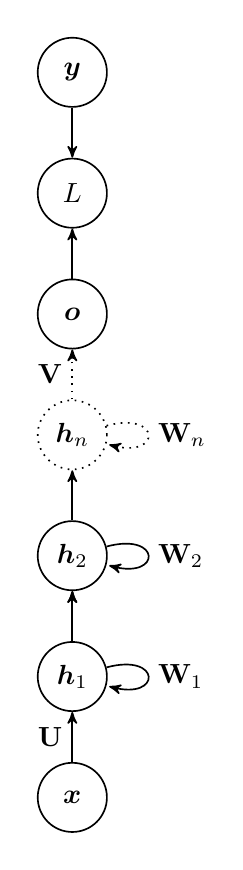
\begin{tikzpicture}[->,>=stealth'
  ,shorten >=0pt
  ,auto,node distance=2.8cm,
  semithick]
  \tikzstyle{every state}=[]

  \matrix (m) [matrix of nodes
  ,row sep=.25in,column sep=.25in] {
    \node[state](y) {$\vc{y}$}; \\
    \node[state](L) {$L$}; \\
    \node[state](o) {$\vc{o}$}; \\
    \node[state,dotted](hn) {$\vc{h}_n$}; \\
    \node[state](h2) {$\vc{h}_2$}; \\
    \node[state](h1) {$\vc{h}_1$}; \\
    \node[state](x) {$\vc{x}$}; \\
  };

  \path
  (x)  edge   node            {$\mt{U}$}   (h1)
  (h1) edge [loop right] node {$\mt{W}_1$} (h1)
  (h2) edge [loop right] node {$\mt{W}_2$} (h2)
  (h1) edge  node {}                       (h2)
  (h1) edge  node {}                       (h2)
  (h2) edge  node {}                       (hn)
  (o)  edge  node {}                       (L)
  (y)  edge  node {}                       (L)
  ;
  \path [dotted] 
  (hn) edge  node {$\mt{V}$} (o)
  (hn) edge [loop right] node {$\mt{W}_n$} (hn)
  ;
  
\end{tikzpicture}

\end{document}